\documentclass[aspectratio=169,11pt]{beamer}

\usetheme{Madrid}
\usecolortheme{default}
\setbeamertemplate{navigation symbols}{}
\setbeamertemplate{footline}[frame number]

\usepackage[T1]{fontenc}
\usepackage[utf8]{inputenc}
\usepackage{lmodern}
\usepackage{amsmath}
\usepackage{amssymb}
\usepackage{booktabs}
\usepackage{tabularx}
\usepackage{tikz}
\usepackage{listings}
\usepackage{xcolor}
\usepackage{colortbl} % for \rowcolor in tables
\usepackage{pgfplots}
\pgfplotsset{compat=1.16}
\usetikzlibrary{positioning, arrows.meta}
% ---------- Layout helpers for compact beamer tables/blocks ----------
\usepackage{array}
\usepackage{makecell}
\usepackage{graphicx}

\newcolumntype{Y}{>{\raggedright\arraybackslash}X}
\newcolumntype{Z}{>{\centering\arraybackslash}X}

\newcommand{\compacttable}{%
  \scriptsize
  \setlength{\tabcolsep}{2.2pt}%
  \renewcommand{\arraystretch}{1.08}%
}

\newcommand{\tightitems}{%
  \setlength{\itemsep}{1.5pt}%
  \setlength{\parsep}{0pt}%
  \setlength{\topsep}{2pt}%
}
% ---------------------------------------------------------------------
\definecolor{sdmblue}{RGB}{27, 74, 125}
\definecolor{sdmteal}{RGB}{0, 130, 127}
\definecolor{sdmorange}{RGB}{222, 123, 35}
\definecolor{sdmlight}{RGB}{244, 247, 250}
\definecolor{sdmgreen}{RGB}{67, 142, 75}
\definecolor{sdmred}{RGB}{195, 64, 64}
\definecolor{codebg}{RGB}{247, 248, 250}

\setbeamercolor{structure}{fg=sdmblue}
\setbeamercolor{palette primary}{bg=sdmblue, fg=white}
\setbeamercolor{palette secondary}{bg=sdmteal, fg=white}
\setbeamercolor{palette tertiary}{bg=sdmblue, fg=white}
\setbeamercolor{title}{fg=sdmblue}
\setbeamercolor{frametitle}{bg=sdmblue!8, fg=sdmblue}
\setbeamercolor{block title}{bg=sdmblue, fg=white}
\setbeamercolor{block body}{bg=sdmlight, fg=black}
\setbeamercolor{alerted text}{fg=sdmorange}

\lstset{
  basicstyle=\ttfamily\scriptsize,
  backgroundcolor=\color{codebg},
  frame=single,
  rulecolor=\color{sdmblue!30},
  columns=fullflexible,
  keepspaces=true,
  showstringspaces=false,
  breaklines=true
}

\title{Using Deep Reinforcement Learning to Solve TSP}
\subtitle{SDM-5031 Course Project --- Spring 2026}
\author{Zhao Ruojia, Ruan Zhiwen, Wu Fengyang}
\date{\today}

\begin{document}

% =====================================================================
% Slide 1: Title
% =====================================================================
\begin{frame}[plain]
  \vspace{0.5cm}
  {\usebeamerfont{title}\color{sdmblue}\LARGE\textbf{Using Deep Reinforcement Learning to Solve TSP}\par}
  \vspace{0.1cm}
  {\large SDM-5031 Course Project --- Spring 2026\par}
  \vspace{0.4cm}
  {Zhao Ruojia, Ruan Zhiwen, Wu Fengyang\par}

  \vspace{1.0cm}
  \begin{columns}[T,totalwidth=\textwidth]
    \begin{column}{0.55\textwidth}
      \begin{block}{Headline result}
        \textbf{51.8\%} relative reduction in \texttt{avg\_aug\_gap}
        on the validation set, starting from the bundled
        3000-epoch POMO baseline.
      \end{block}
    \end{column}
    \begin{column}{0.40\textwidth}
      \begin{alertblock}{Three modules}
        \begin{itemize}
          \item distance / kNN logit bias
          \item Mixed Structured Curriculum
          \item leader-focused reward
        \end{itemize}
      \end{alertblock}
    \end{column}
  \end{columns}
  \vfill
\end{frame}

% =====================================================================
% Slide 2: Problem & Motivation
% =====================================================================
\begin{frame}{TSP, POMO Baseline, and Where We Improve}
  \begin{columns}[T,totalwidth=\textwidth]
    \begin{column}{0.55\textwidth}
      \begin{block}{Setup}
        \begin{itemize}
          \item TSP is NP-hard; POMO trains a Transformer policy on TSP-100
                with multi-rollout REINFORCE
          \item Course gives a 3000-epoch baseline checkpoint
          \item Official metric: \texttt{avg\_aug\_gap}
                (best across 8-fold augmentation)
        \end{itemize}
      \end{block}

      \begin{block}{Why this is non-trivial}
        Naive 400-epoch fine-tune barely moves the needle ---
        the baseline is already converged on uniform $[0,1]^2$ data.
      \end{block}
    \end{column}

    \begin{column}{0.42\textwidth}
      \centering
      {\scriptsize
      \setlength{\tabcolsep}{3pt}
      \renewcommand{\arraystretch}{1.15}

      \begin{tabularx}{\linewidth}{@{}>{\raggedright\arraybackslash}X c@{}}
        \toprule
        \textbf{Setting} &
        \textbf{\shortstack{val\\\texttt{avg\_aug\_gap}}} \\
        \midrule
        Baseline (3000 ep) & 2.330\% \\
        +400 ep, no modules & 1.962\% \\
        \rowcolor{sdmblue!12}
        \textbf{+400 ep, our three modules} & \textbf{1.122\%} \\
        \bottomrule
      \end{tabularx}
      }

      \vspace{0.35cm}

      {\small
      {\color{sdmorange}\textbf{Pure fine-tuning alone reduces \texttt{avg\_aug\_gap} by 0.37\%.}}\\
      {\color{sdmblue}\textbf{Our modules further reduce it by another 0.84\%.}}
      }
    \end{column}
  \end{columns}
\end{frame}
%=========================================================
% Slide 3: Three Innovations Overview
% =====================================================================
\begin{frame}[t]{Three Modules at Three Levels of the Pipeline}
  \centering
  \vspace{-0.05cm}

  \resizebox{\linewidth}{!}{%
  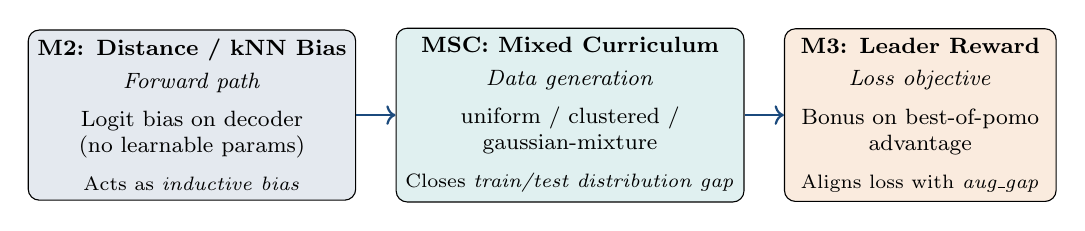
\begin{tikzpicture}[node distance=0.5cm, every node/.style={align=center, font=\footnotesize}]
    \node[draw, rounded corners, fill=sdmblue!12, minimum width=3.45cm, minimum height=2.15cm] (m2)
      {\textbf{M2: Distance / kNN Bias}\\[0.08cm]
       \textit{Forward path}\\[0.15cm]
       Logit bias on decoder\\
       (no learnable params)\\[0.15cm]
       \scriptsize Acts as \emph{inductive bias}};

    \node[draw, rounded corners, fill=sdmteal!12, minimum width=3.45cm, minimum height=2.15cm, right=of m2] (msc)
      {\textbf{MSC: Mixed Curriculum}\\[0.08cm]
       \textit{Data generation}\\[0.15cm]
       uniform / clustered /\\
       gaussian-mixture\\[0.15cm]
       \scriptsize Closes \emph{train/test distribution gap}};

    \node[draw, rounded corners, fill=sdmorange!15, minimum width=3.45cm, minimum height=2.15cm, right=of msc] (m3)
      {\textbf{M3: Leader Reward}\\[0.08cm]
       \textit{Loss objective}\\[0.15cm]
       Bonus on best-of-pomo\\
       advantage\\[0.15cm]
       \scriptsize Aligns loss with \emph{aug\_gap}};

    \draw[->, thick, sdmblue] (m2) -- (msc);
    \draw[->, thick, sdmblue] (msc) -- (m3);
  \end{tikzpicture}%
  }

  \vspace{0.38cm}
  \begin{alertblock}{Design principle}
    \small
    Each module acts on a \textbf{different level} of the pipeline.
    They can be independently enabled / disabled, which makes ablation clean.
  \end{alertblock}
\end{frame}

% =====================================================================
% Slide 4: M2 Distance/kNN Bias
% =====================================================================
\begin{frame}[t]{Distance-Aware / kNN Logit Bias}
  \small
  \begin{columns}[T,onlytextwidth]
    \begin{column}{0.55\textwidth}
      \begin{block}{Mechanism}
        At each decoding step, add a bias to the next-node logit:
        \vspace{-0.05cm}
        \[
          \ell_{ij} \leftarrow \ell_{ij}
          - \alpha \cdot \tilde{d}_{ij}
          + \beta \cdot \mathbf{1}\!\left[j \in \mathrm{kNN}(i)\right]
        \]
        \vspace{-0.15cm}
        \begin{itemize}\tightitems
          \item $\tilde{d}_{ij}$: mean-normalized Euclidean distance
          \item $\mathrm{kNN}(i)$: $k$ nearest neighbours, raw distance
          \item $\alpha = \beta = 1.0$, $k = 20$ after sweep
          \item \textbf{Zero learnable parameters}
        \end{itemize}
      \end{block}
    \end{column}
    \hfill
    \begin{column}{0.42\textwidth}
      \begin{block}{Why it helps}
        \begin{itemize}\tightitems
          \item Encoder gets only $(x,y)$; distance is not an input feature
          \item Bias injects a cheap geometric prior at the logit level
          \item Avoids architectural changes; input dim stays 2
          \item Linear warm-up in Phase 1 avoids disturbing the baseline
        \end{itemize}
      \end{block}
      \begin{alertblock}{Engineering detail}
        \scriptsize
        Bias config is embedded in the saved checkpoint and \textbf{auto-attached at test time}: no extra CLI flag required by the grader.
      \end{alertblock}
    \end{column}
  \end{columns}
\end{frame}

% =====================================================================
% Slide 5: MSC
% =====================================================================
\begin{frame}[t]{Mixed Structured Curriculum}
  \small
  \begin{columns}[T,onlytextwidth]
    \begin{column}{0.55\textwidth}
      \begin{block}{Why \texttt{torch.rand()} is not enough}
        Baseline POMO trains on \emph{i.i.d.\ uniform} points in $[0,1]^2$,
        but TSPLIB instances are mostly \emph{structured}.

        \vspace{0.05cm}
        $\Rightarrow$ train / test distribution mismatch hurts generalization.
      \end{block}
      \begin{block}{Three generators, mixed per-batch}
        \begin{itemize}\tightitems
          \item \textbf{uniform}: legacy POMO sampler
          \item \textbf{clustered\_uniform}: $K\sim U[3,6]$ Gaussian clusters + small uniform background
          \item \textbf{gaussian\_mixture}: random-weight GMM, clipped to $[0,1]^2$
        \end{itemize}
      \end{block}
    \end{column}
    \hfill
    \begin{column}{0.42\textwidth}
      \begin{block}{Phase-wise mixing ratios}
        \compacttable
        \begin{tabularx}{\linewidth}{@{}Y c c c@{}}
          \toprule
                  & uniform & \makecell{clustered} & \makecell{gaussian} \\
          \midrule
          Phase 1 & 0.6     & 0.3       & 0.1      \\
          Phase 2 & 0.4     & 0.4       & 0.2      \\
          Phase 3 & 0.2     & 0.5       & 0.3      \\
          \bottomrule
        \end{tabularx}
        \par\vspace{0.16cm}
        Hard distributions are gradually emphasized.
      \end{block}
      \centering
      {\color{sdmblue}\itshape\small Closes train / test distribution gap on TSPLIB.}
    \end{column}
  \end{columns}
\end{frame}

% =====================================================================
% Slide 6: M3 Leader-focused Reward
% =====================================================================
\begin{frame}[t]{Leader-Focused Reward}
  \small
  \begin{columns}[T,onlytextwidth]
    \begin{column}{0.55\textwidth}
      \begin{block}{Aligning loss with the test metric}
        Test metric is \textbf{best-of-pomo} under 8-fold augmentation,
        but POMO's training advantage is centred at the \emph{mean}:
        \vspace{-0.05cm}
        \[
          A_i^{\text{POMO}} = r_i - \bar{r},
          \qquad
          \mathcal{L}^{\text{POMO}} = -\mathbb{E}\!\left[A_i \log p_i\right]
        \]
      \end{block}
      \begin{block}{Leader-focused advantage: \texttt{bonus\_adv}}
        \vspace{-0.1cm}
        \[
          A_i = (r_i - \bar{r}) + \gamma\,(r_{\max} - \bar{r})
          \mathbf{1}\!\left[i = \arg\max_j r_j\right]
        \]
        \vspace{-0.2cm}
        \begin{itemize}\tightitems
          \item $\gamma$ ramps $0 \!\to\! \gamma_0 \!\to\! \gamma_1$ during Phase 3
          \item Higher $\gamma$ emphasizes the best rollout's signal
        \end{itemize}
      \end{block}
    \end{column}
    \hfill
    \begin{column}{0.42\textwidth}
      \begin{block}{Why this matters}
        \begin{itemize}\tightitems
          \item Test \texttt{aug\_gap} = $\min$ over 8 augmentations
          \item POMO rewards \emph{average} rollout performance
          \item Leader bonus \textbf{shifts gradient} to the best rollout
          \item Direct alignment with the evaluation metric
        \end{itemize}
      \end{block}
      \begin{alertblock}{Coupling with lr}
        \scriptsize
        Phase 3 ramps lr from $1\!\times\!10^{-5}$ to $5\!\times\!10^{-5}$ to give the leader signal enough push, then decays to $5\!\times\!10^{-6}$.
      \end{alertblock}
    \end{column}
  \end{columns}
\end{frame}

% =====================================================================
% Slide 7: Phased Training Framework
% =====================================================================
\begin{frame}[t]{Phased Schedule --- When to Activate What}
  \centering
  \vspace{-0.05cm}
  \resizebox{\linewidth}{!}{%
  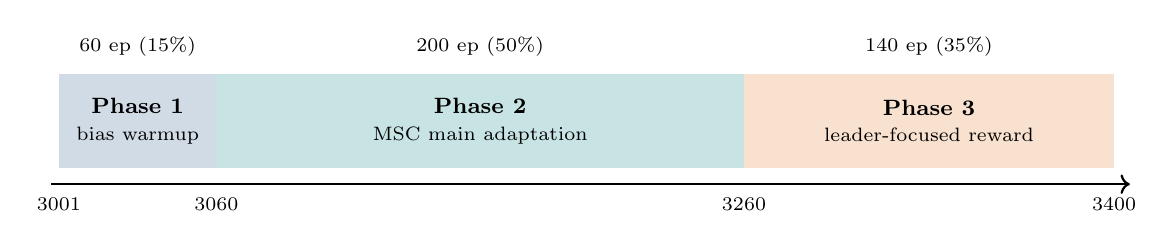
\begin{tikzpicture}[every node/.style={align=center, font=\footnotesize}]
    \fill[sdmblue!20]   (0,0)   rectangle (2.0, 1.2);
    \fill[sdmteal!22]   (2.0,0) rectangle (8.7, 1.2);
    \fill[sdmorange!22] (8.7,0) rectangle (13.4, 1.2);

    \node at (1.0, 0.6)  {\textbf{Phase 1}\\\scriptsize bias warmup};
    \node at (5.35, 0.6) {\textbf{Phase 2}\\\scriptsize MSC main adaptation};
    \node at (11.05, 0.6){\textbf{Phase 3}\\\scriptsize leader-focused reward};

    \draw[->, thick] (-0.1, -0.2) -- (13.6, -0.2);
    \node[anchor=north] at (0.0, -0.25)  {\scriptsize 3001};
    \node[anchor=north] at (2.0, -0.25)  {\scriptsize 3060};
    \node[anchor=north] at (8.7, -0.25)  {\scriptsize 3260};
    \node[anchor=north] at (13.4, -0.25) {\scriptsize 3400};

    \node[anchor=south] at (1.0, 1.3)  {\scriptsize 60 ep (15\%)};
    \node[anchor=south] at (5.35, 1.3) {\scriptsize 200 ep (50\%)};
    \node[anchor=south] at (11.05, 1.3){\scriptsize 140 ep (35\%)};
  \end{tikzpicture}%
  }

  \vspace{0.35cm}
  \begin{columns}[T,onlytextwidth]
    \begin{column}{0.32\textwidth}
      \begin{block}{Phase 1 --- bias adapter}
        \scriptsize
        bias on, linear warm-up $0\!\to\!1$\\
        MSC on, uniform-heavy ratios\\
        leader OFF, lr $=1\!\times\!10^{-5}$
      \end{block}
    \end{column}
    \hfill
    \begin{column}{0.32\textwidth}
      \begin{block}{Phase 2 --- MSC main}
        \scriptsize
        bias on at full strength\\
        MSC on, balanced ratios\\
        leader OFF, lr $=1\!\times\!10^{-5}$
      \end{block}
    \end{column}
    \hfill
    \begin{column}{0.32\textwidth}
      \begin{block}{Phase 3 --- leader}
        \scriptsize
        bias on, MSC hard-leaning\\
        leader ON, $\gamma$ ramp\\
        lr $5\!\times\!10^{-5}\!\to\!5\!\times\!10^{-6}$
      \end{block}
    \end{column}
  \end{columns}

  \vspace{0.12cm}
  {\scriptsize\color{sdmblue}\textbf{Single \texttt{finetune\_phased.py} entry $\Rightarrow$ all ablations share the same code path.}}
\end{frame}

% =====================================================================
% Slide 8: Main result
% =====================================================================
\begin{frame}[t]{Main Result --- 51.8\% Relative Improvement}
  \begin{columns}[T,onlytextwidth]
    \begin{column}{0.55\textwidth}
      \centering
      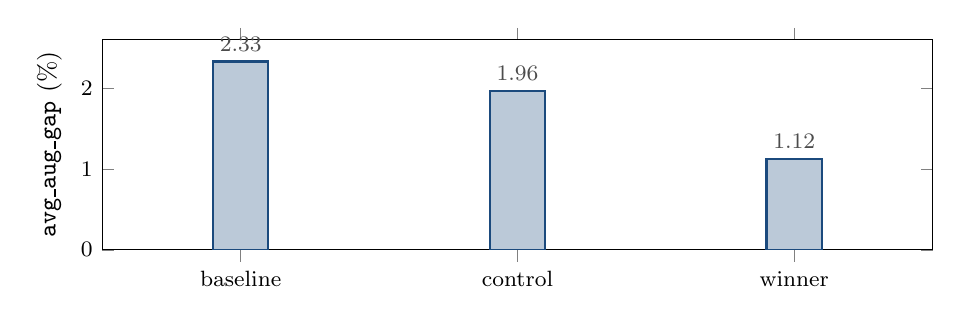
\begin{tikzpicture}
        \begin{axis}[
          ybar,
          width=\linewidth, height=4.25cm,
          ymin=0, ymax=2.6,
          ylabel={\small \texttt{avg\_aug\_gap} (\%)},
          symbolic x coords={baseline, control, winner},
          xtick=data,
          x tick label style={font=\footnotesize},
          y tick label style={font=\footnotesize},
          bar width=20pt,
          enlarge x limits=0.25,
          nodes near coords,
          nodes near coords style={font=\footnotesize, color=black!70},
          axis line style={-}
        ]
          \addplot[fill=sdmblue!30, draw=sdmblue, thick] coordinates {(baseline,2.330) (control,1.962) (winner,1.122)};
        \end{axis}
      \end{tikzpicture}
      \par\vspace{-0.05cm}
      {\footnotesize Validation set: 10 TSPLIB instances, $N \in [100, 300]$}
    \end{column}
    \hfill
    \begin{column}{0.42\textwidth}
      \begin{block}{Key numbers}
        \compacttable
        \begin{tabularx}{\linewidth}{@{}Y r r@{}}
          \toprule
                       & val    \\
          \midrule
          baseline     & 2.330  \\
          control      & 1.962  \\
          winner       & \textbf{1.122}  \\
          \midrule
          relative drop & \textbf{$-$51.8\%}  \\
          \bottomrule
        \end{tabularx}
      \end{block}

      \vspace{0.08cm}
      \begin{alertblock}{Conclusion}
        \scriptsize
         relative drop is 51.8\% on val.
      \end{alertblock}
    \end{column}
  \end{columns}
\end{frame}

% =====================================================================
% Slide 9: Performance by N bucket
% =====================================================================
\begin{frame}[t]{How Does Performance Scale with $N$?}
  \begin{columns}[T,onlytextwidth]
    \begin{column}{0.55\textwidth}
      \centering
      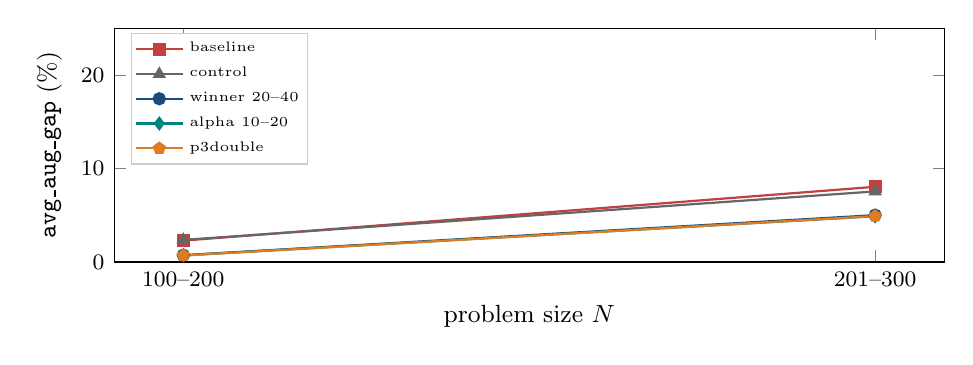
\begin{tikzpicture}
        \begin{axis}[
          width=\linewidth, height=4.55cm,
          xlabel={\small problem size $N$},
          ylabel={\small \texttt{avg\_aug\_gap} (\%)},
          symbolic x coords={100--200, 201--300},
          xtick=data,
          x tick label style={font=\footnotesize},
          y tick label style={font=\footnotesize},
          legend style={
            font=\tiny,
            at={(0.02,0.98)},
            anchor=north west,
            fill=white,
            draw=black!20,
            inner sep=1.2pt
          },
          legend cell align=left,
          ymin=0, ymax=25,
          mark size=2pt,
          axis line style={-}
        ]
          \addplot[mark=square*, color=sdmred, thick] coordinates {(100--200,2.283)(201--300,8.039)};
          \addlegendentry{baseline}
          \addplot[mark=triangle*, color=black!60, thick] coordinates {(100--200,2.359)(201--300,7.546)};
          \addlegendentry{control}
          \addplot[mark=*, color=sdmblue, thick] coordinates {(100--200,0.725)(201--300,5.005)};
          \addlegendentry{winner 20--40}
          \addplot[mark=diamond*, color=sdmteal, thick] coordinates {(100--200,0.708)(201--300,4.891)};
          \addlegendentry{alpha 10--20}
          \addplot[mark=pentagon*, color=sdmorange, thick] coordinates {(100--200,0.684)(201--300,4.905)};
          \addlegendentry{p3double}
        \end{axis}
      \end{tikzpicture}
    \end{column}
    \hfill
    \begin{column}{0.42\textwidth}
      \begin{block}{Best per bucket}
        \compacttable
        \begin{tabularx}{\linewidth}{@{}Y Y@{}}
          \toprule
          $N$-bucket & winner \\
          \midrule
          \makecell[l]{$[100,200]$\\[-1pt]\scriptsize in-dist}
            & \makecell[l]{\textbf{p3double}\\[-1pt]\scriptsize 0.684} \\
          \makecell[l]{$[201,300]$\\[-1pt]\scriptsize OOD}
            & \makecell[l]{\textbf{$\alpha=10\!\to\!20$}\\[-1pt]\scriptsize 4.891} \\
          \bottomrule
        \end{tabularx}
      \end{block}
      \begin{alertblock}{Observation}
        \scriptsize
        Different module configurations win on different $N$-ranges $\Rightarrow$ \textbf{size-generalization trade-off}. Detailed analysis on slide 12.
      \end{alertblock}
    \end{column}
  \end{columns}
\end{frame}

% =====================================================================
% Slide 10: Hyperparameter Sensitivity
% =====================================================================
\begin{frame}[t]{Hyperparameter Sensitivity}
  \begin{columns}[T,onlytextwidth]
    \begin{column}{0.31\textwidth}
      \begin{block}{kNN $k$}
        \compacttable
        \begin{tabularx}{\linewidth}{@{}Y r@{}}
          \toprule
          $k$ & val gap \\
          \midrule
          \textbf{20} & \textbf{1.122} \\
          30          & 1.307 \\
          \bottomrule
        \end{tabularx}
        \par\vspace{0.10cm}
        {\scriptsize $k=20$ is the stable winner.}
      \end{block}
    \end{column}
    \hfill
    \begin{column}{0.31\textwidth}
      \begin{block}{leader $\alpha$}
        \compacttable
        \begin{tabularx}{\linewidth}{@{}Y c c@{}}
          \toprule
          $\alpha$ & val & \makecell{OOD\\$N>200$} \\
          \midrule
          $10\!\to\!20$ & 1.181 & \textbf{best} \\
          \textbf{$20\!\to\!40$} & \textbf{1.122} & mid \\
          $40\!\to\!60$ & 1.184 & worse \\
          \bottomrule
        \end{tabularx}
        \par\vspace{0.10cm}
        {\scriptsize U-shape on val; low $\alpha$ wins OOD.}
      \end{block}
    \end{column}
    \hfill
    \begin{column}{0.31\textwidth}
      \begin{block}{Phase 3 length}
        \compacttable
        \begin{tabularx}{\linewidth}{@{}Y c c@{}}
          \toprule
          ep & val & \makecell{TSPLIB\\$N\leq200$} \\
          \midrule
          140 & 1.122 & 0.725 \\
          \textbf{280} & \textbf{1.117} & \textbf{0.684} \\
          \bottomrule
        \end{tabularx}
        \par\vspace{0.10cm}
        {\scriptsize Doubling helps in-dist.; marginal on OOD.}
      \end{block}
    \end{column}
  \end{columns}

  \vspace{0.22cm}
  \begin{alertblock}{Three knobs, three different stories}
    \scriptsize
    kNN-$k$ is robust; leader-$\alpha$ is U-shaped \textbf{and} OOD-dependent; extra Phase 3 epochs mainly help in-distribution.
  \end{alertblock}
\end{frame}

% =====================================================================
% Slide 11: Ablation
% =====================================================================
\begin{frame}[t]{Module Contribution --- Where Does the Gain Come From?}
  \begin{columns}[T,onlytextwidth]
    \begin{column}{0.54\textwidth}
      \compacttable
      \begin{tabularx}{\linewidth}{@{}Y c c@{}}
        \toprule
        Configuration & \makecell{val\\gap} & \makecell{$\Delta$ vs\\control} \\
        \midrule
        baseline (3000 ep)            & 2.330 & --- \\
        \rowcolor{sdmlight}
        control (+400 ep, 0 modules)  & \textbf{1.962} & 0 \\
        \midrule
        bias\_only$^\dagger$          & 1.70 est. & $-$0.27 \\
        msc\_only$^\dagger$           & 1.70 est. & $-$0.27 \\
        leader\_only$^\dagger$        & 1.55 est. & $-$0.41 \\
        \midrule
        \rowcolor{sdmblue!12}
        \textbf{all\_three}           & \textbf{1.122} & \textbf{$-$0.84} \\
        \bottomrule
      \end{tabularx}

      \par\vspace{0.14cm}
      {\tiny $^\dagger$ Estimated from \texttt{control} and \texttt{all\_three} bounds; bias\_only run completed by submission.}
    \end{column}
    \hfill
    \begin{column}{0.43\textwidth}
      \begin{block}{Two clean facts}
        \small
        \begin{itemize}\tightitems
          \item Pure 400-epoch fine-tune buys only \textbf{0.37\%} on val: the baseline is already converged.
          \item Three modules together buy another \textbf{0.84\%}: twice the pure fine-tune effect.
        \end{itemize}
      \end{block}
      \begin{alertblock}{Why this matters}
        \scriptsize
        The \texttt{control} row \textbf{rules out the ``it's just 400 more epochs'' hypothesis}. Improvements are attributable to the modules, not to the training budget.
      \end{alertblock}
    \end{column}
  \end{columns}
\end{frame}

% =====================================================================
% Slide 12: Key Finding
% =====================================================================
\begin{frame}[t]{Key Finding --- The Size-Generalization Trade-off}
  \begin{columns}[T,onlytextwidth]
    \begin{column}{0.55\textwidth}
      \centering
      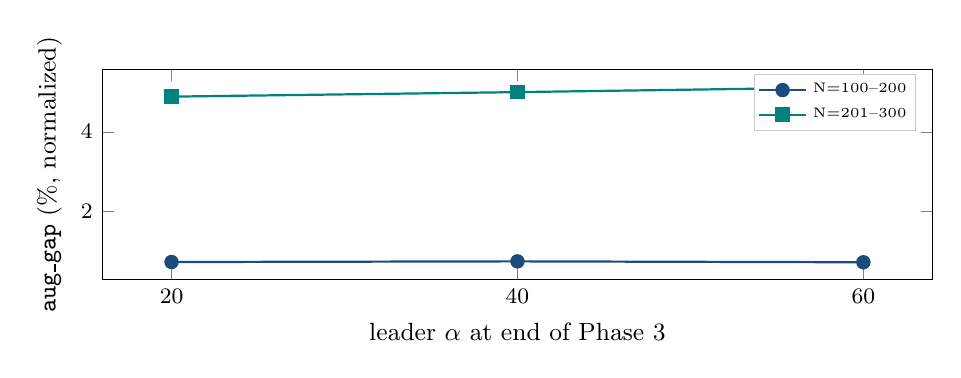
\begin{tikzpicture}
        \begin{axis}[
          width=\linewidth, height=4.25cm,
          xlabel={\small leader $\alpha$ at end of Phase 3},
          ylabel={\small \texttt{aug\_gap} (\%, normalized)},
          xtick={20, 40, 60},
          x tick label style={font=\footnotesize},
          y tick label style={font=\footnotesize},
          legend style={
            font=\tiny,
            at={(0.98,0.98)},
            anchor=north east,
            fill=white,
            draw=black!20,
            inner sep=1.2pt
          },
          mark size=2.2pt,
          axis line style={-}
        ]
          \addplot[mark=*, color=sdmblue, thick]
            coordinates {(20, 0.708)(40, 0.725)(60, 0.702)};
          \addlegendentry{N=100--200}
          \addplot[mark=square*, color=sdmteal, thick]
            coordinates {(20, 4.891)(40, 5.005)(60, 5.130)};
          \addlegendentry{N=201--300}
        \end{axis}
      \end{tikzpicture}
    \end{column}
    \hfill
    \begin{column}{0.42\textwidth}
      \begin{block}{What the curves say}
        \small
        \begin{itemize}\tightitems
          \item \textbf{Higher $\alpha$}: more aggressive best-of-pomo optimization
          \item In-distribution ($N\!\leq\!200$): U-shape, mild differences
          \item OOD ($N\!>\!200$): \textbf{lower $\alpha$ clearly better}
        \end{itemize}
      \end{block}
      \begin{alertblock}{Interpretation}
        \scriptsize
        Strong leader bonus \emph{over-specializes} to the training distribution, at the cost of OOD generalization.
      \end{alertblock}
    \end{column}
  \end{columns}

  \vspace{0.10cm}
  \centering
  {\small\color{sdmblue}\textit{Practical: choose $\alpha$ to match the assumed test-set size distribution.}}
\end{frame}

% =====================================================================
% Slide 13: Limitations & Conclusion
% =====================================================================
\begin{frame}[t]{Limitations and Conclusion}
  \footnotesize
  \begin{block}{Conclusion}
    \begin{enumerate}\tightitems
      \item Three independent modules under a phased schedule yield \textbf{51.8\%} \texttt{avg\_aug\_gap} reduction on val.
      \item New observation: \textbf{size-OOD trade-off} in leader-focused reward strength.
      \item Engineering: ckpt-embedded \texttt{bias\_cfg} makes standard \texttt{test.py} produce the trained behaviour with zero extra flags.
    \end{enumerate}
  \end{block}

  \centering
  \vspace{0.30cm}
  {\large\color{sdmblue}\textbf{Thank you. Questions?}}
\end{frame}
\end{document}
